%% bare_jrnl_compsoc.tex
%% V1.4b
%% 2015/08/26
%% by Michael Shell
%% See:
%% http://www.michaelshell.org/
%% for current contact information.
%%
%% This is a skeleton file demonstrating the use of IEEEtran.cls
%% (requires IEEEtran.cls version 1.8b or later) with an IEEE
%% Computer Society journal paper.
%%
%% Support sites:
%% http://www.michaelshell.org/tex/ieeetran/
%% http://www.ctan.org/pkg/ieeetran
%% and
%% http://www.ieee.org/

% *** Authors should verify (and, if needed, correct) their LaTeX system  ***
% *** with the testflow diagnostic prior to trusting their LaTeX platform ***
% *** with production work. The IEEE's font choices and paper sizes can   ***
% *** trigger bugs that do not appear when using other class files.       ***                          ***
% The testflow support page is at:
% http://www.michaelshell.org/tex/testflow/


\documentclass[10pt,journal,compsoc]{IEEEtran}
%
% If IEEEtran.cls has not been installed into the LaTeX system files,
% manually specify the path to it like:
% \documentclass[10pt,journal,compsoc]{../sty/IEEEtran}

% *** CITATION PACKAGES ***
%
\ifCLASSOPTIONcompsoc
  % IEEE Computer Society needs nocompress option
  % requires cite.sty v4.0 or later (November 2003)
  \usepackage[nocompress]{cite}
\else
  % normal IEEE
  \usepackage{cite}
\fi

% *** GRAPHICS RELATED PACKAGES ***
%
\ifCLASSINFOpdf
  \usepackage[pdftex]{graphicx}
\else
  \usepackage[dvips]{graphicx}
\fi

% *** MATH PACKAGES ***
\usepackage{amsmath,amssymb,amsfonts}

% *** SPECIALIZED LIST PACKAGES ***
\usepackage{algorithmic}

% *** ALIGNMENT PACKAGES ***
\usepackage{array}

% *** SUBFIGURE PACKAGES ***
\ifCLASSOPTIONcompsoc
  \usepackage[caption=false,font=footnotesize,labelfont=sf,textfont=sf]{subfig}
\else
  \usepackage[caption=false,font=footnotesize]{subfig}
\fi

% *** OTHER PACKAGES ***
\usepackage{textcomp}
\usepackage{xcolor}
\usepackage[utf8]{inputenc}
\usepackage[T1]{fontenc}
\usepackage[polish]{babel}
\usepackage{float}

% correct bad hyphenation here
\hyphenation{op-tical net-works semi-conduc-tor}


\begin{document}
%
% paper title
% Titles are generally capitalized except for words such as a, an, and, as,
% at, but, by, for, in, nor, of, on, or, the, to and up, which are usually
% not capitalized unless they are the first or last word of the title.
% Linebreaks \\ can be used within to get better formatting as desired.
% Do not put math or special symbols in the title.
\title{Objaśnialna Sztuczna Inteligencja (XAI) w Modelach Klasyfikacji PyTorch}

% author names and IEEE memberships
% note positions of commas and nonbreaking spaces ( ~ ) LaTeX will not break
% a structure at a ~ so this keeps an author's name from being broken across
% two lines.
\author{Kacper Witek, Kacper Przybylski% <-this % stops a space
\IEEEcompsocitemizethanks{\IEEEcompsocthanksitem Autorzy są studentami Wydziału FTIMS, Uczelnia Politechnika Łódzka.\protect\\
}% <-this % stops an unwanted space
\thanks{Projekt III z przedmiotu Obliczenia inteligentne, czerwiec~2026.}}

% The paper headers
\markboth{Projekt III z przedmiotu Obliczenia inteligentne, czerwiec~2026}%
{Kacper Witek, Kacper Przybylski: Objaśnialna Sztuczna Inteligencja (XAI) w Modelach Klasyfikacji PyTorch}

% for Computer Society papers, we must declare the abstract and index terms
% PRIOR to the title within the \IEEEtitleabstractindextext IEEEtran
% command as these need to go into the title area created by \maketitle.
% As a general rule, do not put math, special symbols or citations
% in the abstract or keywords.
\IEEEtitleabstractindextext{%
\begin{abstract}
W niniejszym artykule przedstawiono próbę wyjaśnienia procesów decyzyjnych w wybranych modelach sztucznych sieci neuronowych. Zastosowano bibliotekę Captum w celu zbadania zachowań modeli dla zbiorów danych różnego typu: tabelarycznych (Iris, Wine), oraz obrazowych (MNIST, Imagenette). Otrzymane wyniki, oparte o wiele wariantów próbek i klas, wskazują, że metody XAI pozwalają zidentyfikować krytyczne atrybuty decyzyjne oraz dogłębnie ocenić wiarygodność działania skomplikowanych modeli typu "black box".
\end{abstract}

% Note that keywords are not normally used for peerreview papers.
\begin{IEEEkeywords}
XAI, Explainable AI, Captum, PyTorch, LIME, Saliency, Ablation
\end{IEEEkeywords}}


% make the title area
\maketitle


% To allow for easy dual compilation without having to reenter the
% abstract/keywords data, the \IEEEtitleabstractindextext text will
% not be used in maketitle, but will appear (i.e., to be "transported")
% here as \IEEEdisplaynontitleabstractindextext when the compsoc 
% or transmag modes are not selected <OR> if conference mode is selected 
% - because all conference papers position the abstract like regular
% papers do.
\IEEEdisplaynontitleabstractindextext
% \IEEEdisplaynontitleabstractindextext has no effect when using
% compsoc or transmag under a non-conference mode.


% For peer review papers, you can put extra information on the cover
% page as needed:
% \ifCLASSOPTIONpeerreview
% \begin{center} \bfseries EDICS Category: 3-BBND \end{center}
% \fi
%
% For peerreview papers, this IEEEtran command inserts a page break and
% creates the second title. It will be ignored for other modes.
\IEEEpeerreviewmaketitle


\IEEEraisesectionheading{\section{Wprowadzenie (Introduction)}\label{sec:introduction}}
% Computer Society journal (but not conference!) papers do something unusual
% with the very first section heading (almost always called "Introduction").
% They place it ABOVE the main text! IEEEtran.cls does not automatically do
% this for you, but you can achieve this effect with the provided
% \IEEEraisesectionheading{} command.

\IEEEPARstart{R}{ozwój} sztucznej inteligencji, w szczególności uczenia głębokiego (ang. \textit{Deep Learning}), przyczynił się do powstania niezwykle skutecznych, lecz wysoce skomplikowanych modeli decyzyjnych. Sieci te, ze względu na miliony parametrów i nieliniowości, działają zazwyczaj jako tzw. "czarne skrzynki" (ang. \textit{black boxes}). Stanowi to duży problem w dziedzinach krytycznych (np. medycynie, prawie czy finansach), gdzie wysoka dokładność klasyfikacji to za mało. Użytkownik musi wiedzieć, dlaczego model podjął określoną decyzję. Odpowiedzią na te wyzwania jest dziedzina Objaśnialnej Sztucznej Inteligencji (XAI - \textit{Explainable AI}), zajmująca się metodami interpretacji i sprawdzania logiki modeli uczenia maszynowego.

Z punktu widzenia oznaczeń, rozważamy model klasyfikacyjny $f(x)$, który dla danej próbki wejściowej $x$ (np. cech liczbowych lub obrazu) zwraca wynik predykcji. Celem objaśniania lokalnego jest określenie wpływu poszczególnych cech wejściowych $x_i$ na ten wynik. Przypisujemy im wartości atrybucji $a_i$, gdzie wartości dodatnie oznaczają wpływ wspierający decyzję modelu, a wartości ujemne — osłabiający ją. 

Alternatywnym podejściem jest badanie odporności modelu poprzez perturbacje (zaburzenia). Wprowadzamy wówczas zmodyfikowane wejście $\tilde{x} = x + \delta$ i sprawdzamy, przy jakich najmniejszych zmianach $\delta$ model zmieni swoją pierwotną decyzję na inną: $f(\tilde{x}) \neq f(x)$. Pozwala to wyznaczyć granice decyzyjne klasyfikatora.


\section{Powiązane prace (Related Works)}
W dziedzinie XAI rozróżnia się metody specyficzne dla danego modelu (np. oparte o gradienty w sieciach neuronowych) oraz niezależne od modelu (ang. \textit{model-agnostic}, które mogą objaśnić dowolny algorytm). W tym projekcie skupiono się na metodach wyjaśniania lokalnego, które są powszechnie stosowane w literaturze naukowej.

\subsection{Mapy wrażliwości (Saliency Maps)}
Metoda map wrażliwości, wprowadzona przez Simonyana i in. \cite{Simonyan2013}, bazuje na analizie gradientów. Jej celem jest określenie, jak zmiana wartości danego elementu wejścia wpływa na wynik modelu. Matematycznie, dla wejścia $x$ i wyniku danej klasy $S(x)$ wyznacza się gradient:
\begin{equation}
w = \frac{\partial S(x)}{\partial x}
\end{equation}
Wartości tego gradientu mówią nam o lokalnej wrażliwości sieci na drobne zmiany wejścia. W przypadku obrazów kolorowych zazwyczaj wybiera się maksymalną wartość po kanałach barwnych, aby otrzymać jedną czytelną mapę pikseli.

\subsection{LIME (Local Interpretable Model-agnostic Explanations)}
Metoda LIME \cite{Ribeiro2016} działa niezależnie od architektury modelu. Zakłada ona, że choć globalna granica decyzyjna skomplikowanego klasyfikatora jest nieliniowa i trudna do zrozumienia, to lokalnie można ją z powodzeniem przybliżyć prostszym, interpretowalnym modelem liniowym $g$.

W tym celu wokół punktu $x$ generuje się losowe perturbacje (np. maskowanie losowych cech lub superpikseli). Następnie zbiera się predykcje oryginalnego modelu dla tych zaburzonych próbek i na tej podstawie uczy się prostą regresję liniową. Współczynniki tej regresji stanowią lokalne atrybucje istotności cech.

\subsection{Ablacja cech (Feature Ablation)}
Ablacja cech to intuicyjna metoda polegająca na systematycznym wyłączaniu lub zastępowaniu poszczególnych cech wejściowych (lub ich grup) wartościami referencyjnymi (np. zerem) i mierzeniu spadku prawdopodobieństwa poprawnej klasy. Różnica wartości predykcji przed i po usunięciu cechy stanowi jej atrybucję:
\begin{equation}
a_i = f(x) - f(x_{[i \leftarrow 0]})
\end{equation}
Chociaż metoda ta wymaga wielokrotnego uruchamiania modelu dla każdej cechy, pozwala na prostą ocenę wkładu poszczególnych zmiennych \cite{Zeiler2014}.

\subsection{Przykłady przeciwne (Counterfactuals)}
Metody kontrfaktyczne \cite{Wachter2017} badają stabilność decyzji klasyfikatora poprzez szukanie odpowiedzi na pytanie: ,,jaka minimalna modyfikacja cech wejściowych spowoduje zmianę decyzji modelu na inną?''. Poszukuje się zmodyfikowanego wejścia $\tilde{x}$, które jest geometrycznie jak najbliższe oryginalnemu wejściu $x$, ale dla którego predykcja modelu zmienia się na pożądaną klasę $y'$. Dostarcza to intuicyjnych informacji o granicach decyzyjnych modelu.


\section{Metody (Methods)}
W ramach projektu zaimplementowano procesy objaśniania decyzji modeli klasyfikacyjnych na zbiorach danych tabelarycznych i obrazowych. Skupiono się na powiązaniu wyników eksperymentalnych z prostymi oznaczeniami atrybucji.

\subsection{Badane modele i zbiory danych}
Eksperymenty przeprowadzono w następujących konfiguracjach:
\begin{itemize}
    \item \textbf{Dane tabelaryczne (Iris, Wine i MLP Mnist):} Klasyfikacja oparta na wektorach cech ciągłych. Wykorzystano prosty wielowarstwowy perceptron (MLP).
    \item \textbf{Dane obrazowe (MNIST i Imagenette):} Do klasyfikacji wykorzystano sieci konwolucyjne (CNN) działające bezpośrednio na pikselach (obrazów czarno-białych w MNIST oraz kolorowych RGB w Imagenette).
\end{itemize}

\subsection{Ablacja cech}
Na zbiorach Iris i Wine badano wpływ cech poprzez ich wyzerowanie. Jako wektor referencyjny przyjęto tło zerowe. Atrybucję cechy $i$ dla badanej klasy obliczano jako różnicę predykcji:
\begin{equation}
a_i = f(x)_c - f(x_{[i \leftarrow 0]})_c
\end{equation}
Dodatnia wartość atrybucji oznacza, że obecność cechy zwiększa pewność modelu co do poprawnej klasy $c$.

\subsection{Mapy Saliency dla MNIST}
Wizualizacja Saliency opiera się na wyznaczeniu pochodnej wyniku klasyfikacji względem pikseli. Obliczana mapa reprezentuje wartość bezwzględną gradientu dla każdego piksela:
\begin{equation}
a_i = \left| \frac{\partial S_c(x)}{\partial x_i} \right|
\end{equation}
Wskazuje to, które obszary cyfry wykazują najwyższą czułość przy drobnych zmianach jasności pikseli.

\subsection{Metoda LIME z superpikselami}
Dla obrazów (MNIST i Imagenette) zastosowanie LIME bezpośrednio na pojedynczych pikselach jest nieczytelne. Wprowadzono zatem podział obrazu na superpiksele za pomocą algorytmu SLIC. Cały proces przebiegał następująco:
\begin{enumerate}
    \item Segmentacja obrazu na spójne obszary (superpiksele).
    \item Generowanie zaburzonych próbek poprzez losowe zasłanianie superpikseli (kolorem czarnym w MNIST lub średnim kolorem sąsiedztwa w Imagenette).
    \item Wyuczenie lokalnej regresji liniowej na zebranych predykcjach. Współczynniki wagowe modelu stanowią ostateczne atrybucje dla superpikseli.
\end{enumerate}

\subsection{Kierunkowa analiza perturbacyjna}
Zbadano odporność modelu MNIST na częściowe usunięcie cyfry za pomocą stopniowo nakładanej maski (czarnego paska o wysokości $h$ pikseli). Badano dwa rodzaje przesunięcia maski:
\begin{itemize}
    \item \textbf{Od dołu (bottom squeeze):} Zerowanie dolnych $h$ wierszy obrazu.
    \item \textbf{Od góry (top squeeze):} Zerowanie górnych $h$ wierszy obrazu.
\end{itemize}
Dla modyfikowanego wejścia obserwowano, przy jakiej wysokości maski model zaczyna się mylić, co pozwala wyznaczyć punkt krytyczny $h_{crit}$.

\subsection{Analiza globalna poprzez agregację wielu próbek}
Objaśnienia lokalne opisują wyłącznie pojedynczą próbkę, przez co na ich podstawie trudno wnioskować o ogólnym, powtarzalnym sposobie rozpoznawania danej klasy. Aby uzyskać obraz globalny, dla każdej klasy modeli obrazowych (MNIST CNN, MNIST MLP zoning oraz Imagenette CNN) wybrano wiele \emph{poprawnie} sklasyfikowanych próbek (po 5 do prezentacji w siatkach oraz do 60 do uśredniania) i zastosowano dwa komplementarne ujęcia:
\begin{itemize}
    \item \textbf{Siatki przykładów (grids):} zestawienie map atrybucji wielu różnych próbek tej samej klasy obok siebie. Pozwala ocenić, czy model stosuje spójny wzorzec niezależnie od wariantu próbki.
    \item \textbf{Mapy uśrednione (mean):} uśrednienie map atrybucji po $n$ próbkach klasy $c$ daje tzw. globalną sygnaturę klasy
    \begin{equation}
    \bar{a}_c = \frac{1}{n}\sum_{j=1}^{n} a^{(j)}_c,
    \end{equation}
    która uwypukla obszary istotne niezależnie od konkretnej próbki. Uśrednianie stosowano dla metod o stałej dziedzinie pikselowej (Saliency oraz ablacja stref $4\times4$); dla metody LIME, w której segmentacja SLIC jest odmienna dla każdego obrazu, ograniczono się do siatek przykładów.
\end{itemize}


\section{Wyniki (Results)}

\subsection{Charakterystyka zbiorów danych i skuteczność modeli}
Przed analizą wyjaśnień metodami XAI zweryfikowano skuteczność klasyfikacyjną wszystkich zaimplementowanych modeli. Szczegółową charakterystykę poszczególnych zbiorów danych oraz wyniki dokładności (ang. \textit{accuracy}) na wydzielonych zbiorach testowych/walidacyjnych zebrano w Tabeli \ref{tab:datasets}.

\begin{table}[htbp]
\caption{Charakterystyka zbiorów danych i wyniki klasyfikacji}
\label{tab:datasets}
\begin{center}
\begin{tabular}{|l|c|c|c|c|}
\hline
\textbf{Zbiór danych} & \textbf{Typ danych} & \textbf{Model} & \textbf{Dokładność} \\
\hline
Iris & Tabelaryczne & MLP & 100,00\% \\
Wine & Tabelaryczne & MLP & 100,00\% \\
MNIST (zoning) & Tabelaryczne & MLP & 85,04\% \\
MNIST & Obrazowe (2D) & CNN & 98,99\% \\
Imagenette & Obrazowe (3D) & CNN & 71,80\% \\
\hline
\end{tabular}
\end{center}
\end{table}

Modele MLP dla prostszych zadań tabelarycznych (Iris, Wine) osiągnęły pełną bezbłędność (100,00\% dokładności), co oznacza optymalne dopasowanie granic decyzyjnych w tych mało wymiarowych przestrzeniach. Model MLP dla strefowanego MNIST (zoning16, gdzie obraz jest redukowany do 16 cech średniej jasności obszarów) uzyskał wynik 85,04\%, co odzwierciedla ograniczenia uproszczonej reprezentacji cech. Głęboka sieć konwolucyjna (CNN) dla pełnego zbioru MNIST osiągnęła wysoki i stabilny wynik 98,99\%. W przypadku zbioru Imagenette (złożone obrazy naturalne o wysokiej rozdzielczości) model CNN osiągnął satysfakcjonującą dokładność na poziomie 71,80\%, co stanowi właściwy punkt wyjścia do analizy interpretowalności.

\subsection{Dane tabelaryczne}
Zastosowanie \textit{Feature Ablation} na reprezentantach różnych klas wskazało ewidentne różnice atrybucyjne. Pozwala to na zidentyfikowanie cech kluczowych dla decyzji modelu MLP.

W przypadku zbioru Iris (zob. Tabela \ref{tab:iris}), model klasyfikując próbkę jako klasę 0 (Iris-setosa) opiera się przede wszystkim na ujemnym wkładzie cech \textit{sepal length} (-3,8293) oraz \textit{petal length} (-1,4697), przy jednoczesnym silnie dodatnim wkładzie \textit{sepal width} (2,9554). Wizualizację atrybucji dla tej klasy przedstawia Rys. \ref{fig:iris_class0}. Z kolei dla klasy 2 (Iris-virginica), co przedstawiono na Rys. \ref{fig:iris_class2}, decydujące znaczenie mają duże dodatnie wartości cech płatka: \textit{petal length} (5,1655) oraz \textit{petal width} (3,9439). Wyniki te pokrywają się z wiedzą botaniczną: irysy klasy setosa cechują się krótkimi i szerokimi płatkami, zaś virginica posiada płatki najdłuższe i najszersze.

\begin{table}[htbp]
\caption{Wartości atrybucji dla poszczególnych klas - zbiór Iris}
\label{tab:iris}
\begin{center}
\begin{tabular}{|l|c|c|c|}
\hline
\textbf{Cecha} & \textbf{Klasa 0} & \textbf{Klasa 1} & \textbf{Klasa 2} \\
\hline
sepal length (cm) & -3.8293 & 0.2412 & 2.8936 \\
sepal width (cm) & 2.9554 & -0.6618 & -0.5489 \\
petal length (cm) & -1.4697 & -1.1076 & 5.1655 \\
petal width (cm) & -0.2126 & -0.9452 & 3.9439 \\
\hline
\end{tabular}
\end{center}
\end{table}

Podobnie dla zbioru Wine (zob. Tabela \ref{tab:wine}), klasyfikacja do poszczególnych klas zależy od zupełnie innych cech fizykochemicznych. Dla klasy 0 (Rys. \ref{fig:wine_class0}) dominujący wpływ wykazuje stężenie \textit{proline} (atrybucja 128,1493), podczas gdy cecha \textit{magnesium} wpływa silnie ujemnie (atrybucja -12,6521). Odwrotnie sytuacja wygląda w klasie 1, gdzie rola \textit{proline} jest ujemna (-2,8192), a \textit{magnesium} stymuluje decyzję dodatnio (9,5168). Świadczy to o tym, że model prawidłowo wyodrębnił kluczowe markery chemiczne definiujące dany szczep wina.

\begin{table}[htbp]
\caption{Wartości atrybucji dla poszczególnych klas - zbiór Wine}
\label{tab:wine}
\begin{center}
\begin{tabular}{|l|c|c|c|}
\hline
\textbf{Cecha} & \textbf{Klasa 0} & \textbf{Klasa 1} & \textbf{Klasa 2} \\
\hline
alcohol & 0.3522 & -1.2487 & 0.1129 \\
malic\_acid & 0.0015 & -0.0869 & 0.1380 \\
ash & 0.0182 & -0.0536 & 0.0120 \\
alcalinity\_of\_ash & -1.5133 & -0.4452 & 2.2970 \\
magnesium & -12.6521 & 9.5168 & 7.4479 \\
total\_phenols & 0.0287 & 0.2210 & 0.0464 \\
flavanoids & 0.2720 & -0.0226 & -0.0565 \\
nonflavanoid\_phenols & -0.0304 & -0.0019 & 0.0588 \\
proanthocyanins & 0.1242 & 0.0259 & -0.0436 \\
color\_intensity & -0.1438 & -0.4685 & 0.6217 \\
hue & 0.1292 & 0.0879 & -0.0398 \\
od280/od315\_of\_diluted\_wines & 0.4713 & 0.1697 & -0.0141 \\
proline & 128.1493 & -2.8192 & -15.8466 \\
\hline
\end{tabular}
\end{center}
\end{table}

\begin{figure}[H]
\centerline{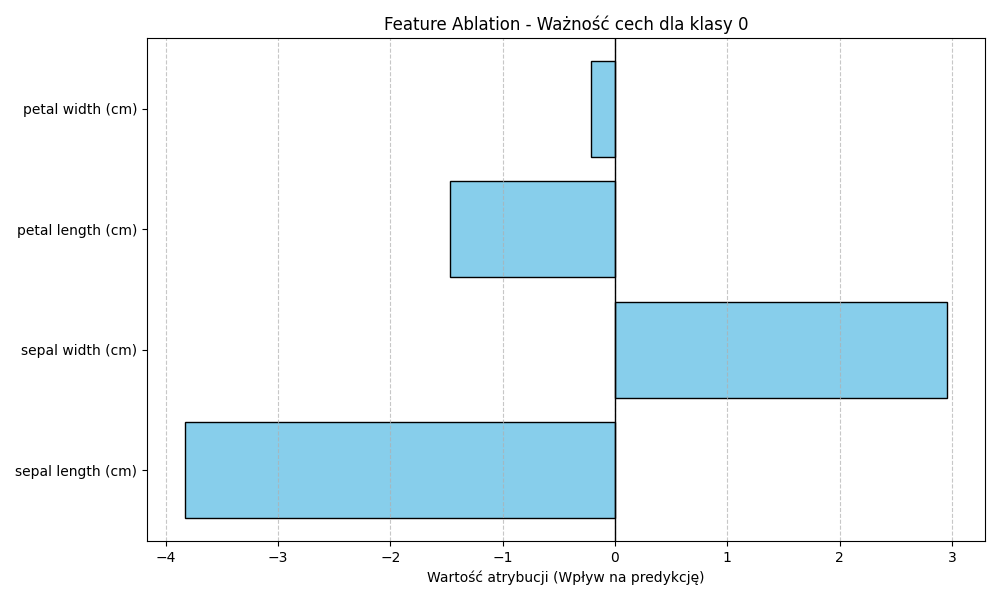
\includegraphics[width=0.45\textwidth]{wyniki_xai/iris_ablation_class0.png}}
\caption{Wpływ cech dla klasy 0 (Iris).}
\label{fig:iris_class0}
\end{figure}
\begin{figure}[H]
\centerline{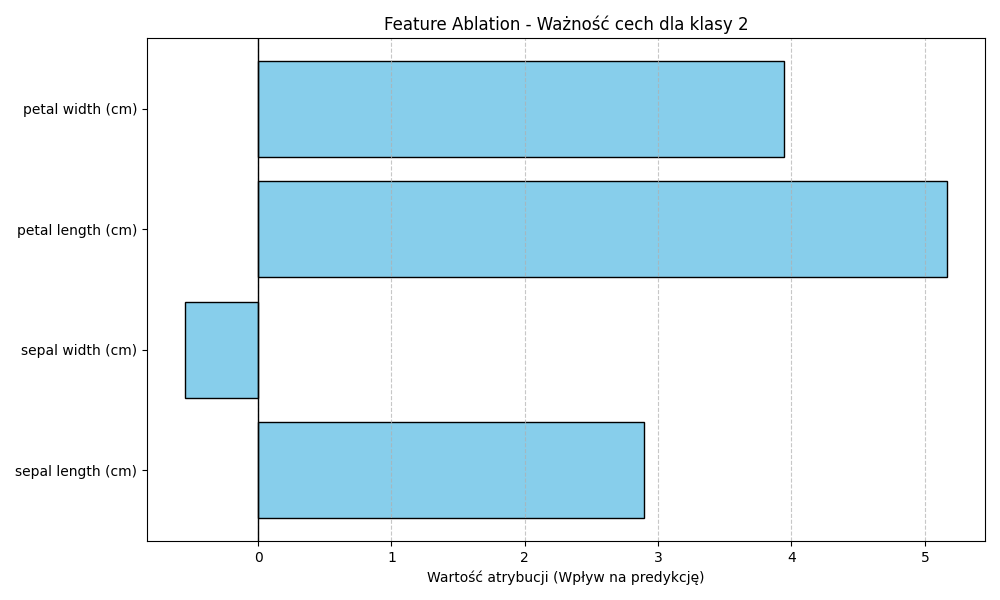
\includegraphics[width=0.45\textwidth]{wyniki_xai/iris_ablation_class2.png}}
\caption{Wpływ cech dla klasy 2 (Iris) - decydująca przewaga płatków.}
\label{fig:iris_class2}
\end{figure}
\begin{figure}[H]
\centerline{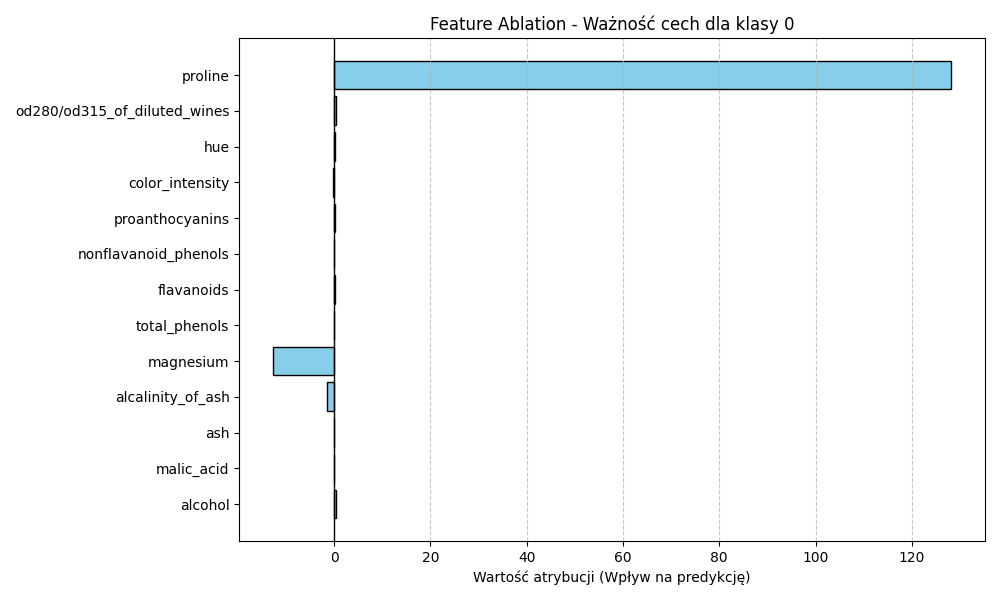
\includegraphics[width=0.45\textwidth]{wyniki_xai/wine_ablation_class0.png}}
\caption{Atrybucja na klasie 0 zbioru Wine.}
\label{fig:wine_class0}
\end{figure}

\subsection{Cyfry pisane odręcznie (MNIST)}
W przypadku zbioru MNIST zanalizowano dwa modele: uproszczony model MLP operujący na 16 cechach strefowych (zoning) oraz głęboki model CNN operujący na pełnym obrazie.

\subsubsection{Model MLP z cechami strefowymi (zoning)}
Dla modelu MLP wejściem jest 16 wartości średniej jasności w siatce $4 \times 4$ stref (gdzie każda strefa to blok o rozmiarze $7 \times 7$ pikseli). Aby lepiej zrozumieć decyzje tego modelu, wektor 16 atrybucji uzyskany metodą \textit{Feature Ablation} przekształcono z powrotem do postaci dwuwymiarowej siatki $4 \times 4$. Wyniki tej wizualizacji dla przykładowej cyfry 7 przedstawiono na Rys. \ref{fig:mnist_mlp_zoning_2d}.

\begin{figure}[H]
\centerline{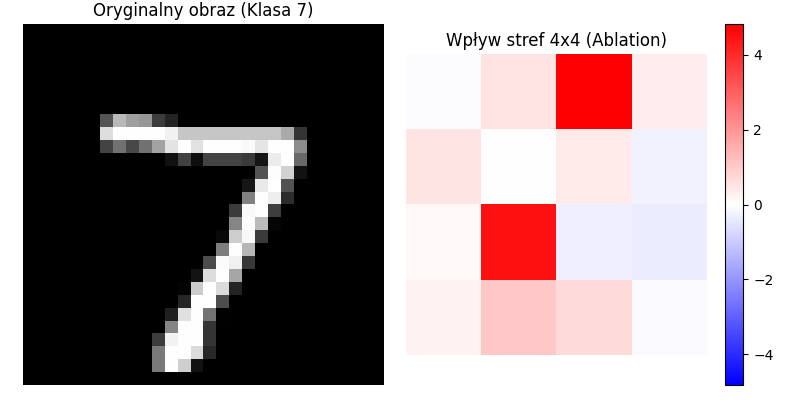
\includegraphics[width=0.45\textwidth]{wyniki_xai/mnist_mlp_zoning_2d.png}}
\caption{Oryginalny obraz cyfry 7 (po lewej) oraz odpowiadająca mu wizualizacja 2D wpływów stref $4 \times 4$ (po prawej) wyznaczona metodą Feature Ablation dla modelu MLP.}
\label{fig:mnist_mlp_zoning_2d}
\end{figure}

Analiza atrybucji strefowych dla cyfry 7 wykazuje, że model MLP opiera swoją decyzję przede wszystkim na dwóch kluczowych obszarach:
\begin{itemize}
    \item \textbf{Strefa 3} (prawy górny róg poziomej kreski cyfry 7) – o silnie dodatniej atrybucji wynoszącej ok. $4{,}82$. Jest to kluczowy element odróżniający cyfrę 7 od innych cyfr (np. od 1).
    \item \textbf{Strefa 10} (środkowo-dolny segment ukośnej kreski cyfry 7) – o atrybucji ok. $4{,}51$, reprezentujący przebieg skośnej linii.
\end{itemize}
Dzięki zrzutowaniu jednowymiarowego wektora cech na siatkę przestrzenną $4 \times 4$, analiza XAI dla modelu tabelarycznego zyskuje intuicyjną interpretację geometryczną, zbliżoną do metod przeznaczonych dla modeli obrazowych.

\subsubsection{Model CNN na pełnym obrazie}
Dla CNN MNIST użyto map atrybucji Saliency, LIME dla superpikseli oraz metody kierunkowych perturbacji maskujących.

Mapa wrażliwości (Saliency Map) dla cyfry 6 (Rys. \ref{fig:mnist_saliency_6}) wykazuje, że gradienty wyjściowego prawdopodobieństwa skupiają się bezpośrednio na linii cyfry, omijając czarne tło. Dowodzi to wrażliwości sieci na rzeczywistą geometrię konturu cyfry.

\begin{figure}[H]
\centerline{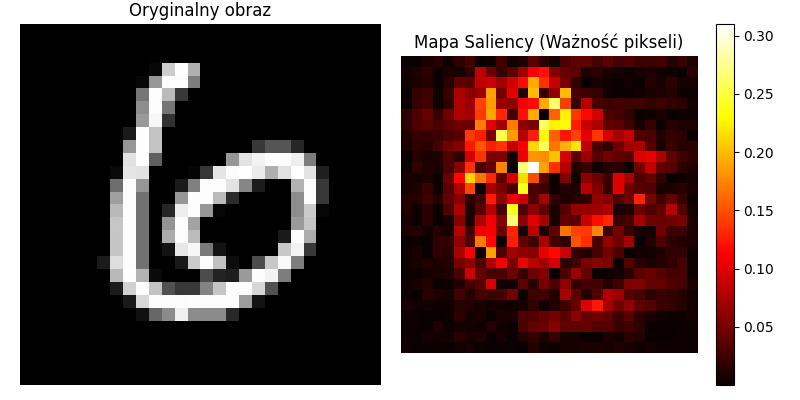
\includegraphics[width=0.45\textwidth]{wyniki_xai/mnist_saliency_sample11_class6.png}}
\caption{Saliency Map dla testowej cyfry 6.}
\label{fig:mnist_saliency_6}
\end{figure}

Wizualizacja perturbacji dolnej dla próbki 33 (cyfra 4) przedstawiona na Rys. \ref{fig:mnist_perturb_6} wskazuje moment deklasyfikacji. Kiedy maska usuwająca (czarny pas od dołu) dociera do wysokości $h=18$ pikseli, dolny kawałek 4 zostaje zamazany. W tym momencie model traci pewność dla cyfry 4 i klasyfikuje pozostałe pionowe kreski jako cyfrę 1. Rys. \ref{fig:mnist_perturb_5} przedstawia analogiczne zachowanie dla cyfry 3: odcięcie dolnej pętli powoduje zmianę predykcji na cyfrę 7. Z kolei dla prostej, pionowej cyfry 1 model okazał się niewrażliwy na deklasyfikację pod wpływem skracania maską, gdyż pozostały fragment zachowywał swój podstawowy osiowy charakter.

\begin{figure}[H]
\centerline{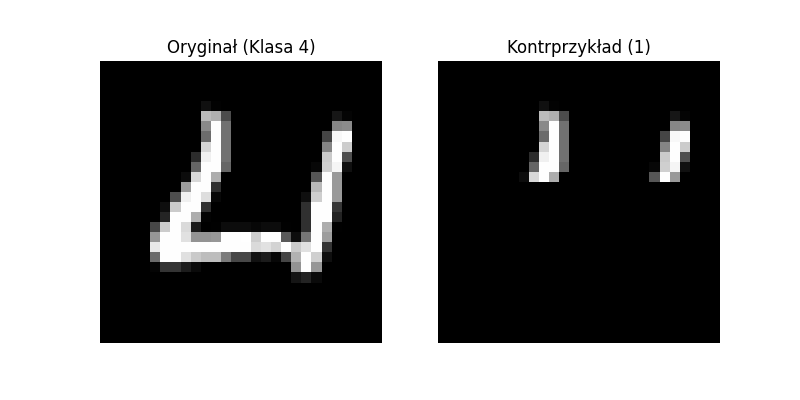
\includegraphics[width=0.45\textwidth]{wyniki_xai/mnist_perturbation_sample33_class4.png}}
\caption{Moment pomylenia uciskanej od dołu cyfry 4 (deklasyfikacja na 1).}
\label{fig:mnist_perturb_6}
\end{figure}
\begin{figure}[H]
\centerline{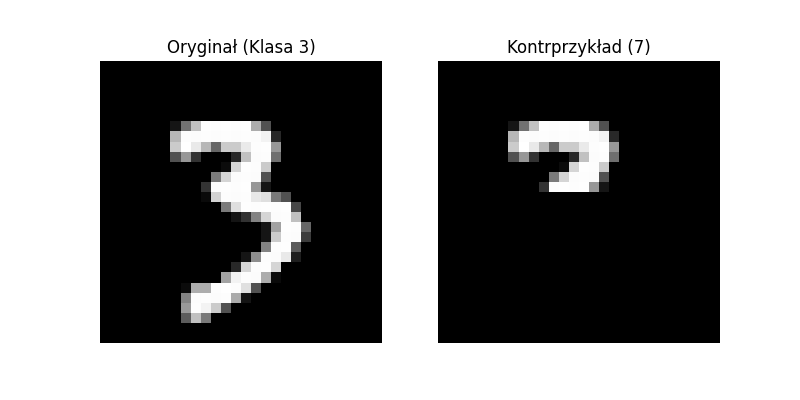
\includegraphics[width=0.45\textwidth]{wyniki_xai/mnist_perturbation_sample30_class3.png}}
\caption{Kontrprzykład dla cyfry 3 - zasłonięcie fragmentu pętli u dołu klasyfikuje rysunek jako 7.}
\label{fig:mnist_perturb_5}
\end{figure}

W analizie opartej o LIME z superpikselami SLIC (Rys. \ref{fig:mnist_lime_3}--\ref{fig:mnist_lime_5}) zaobserwowano, które regiony wspierają (kolor czerwony) lub tłumią (kolor niebieski) poprawną klasę. Dla cyfry 3 (Rys. \ref{fig:mnist_lime_3}) kluczowy wpływ mają superpiksele tworzące charakterystyczne łuki. Dla cyfry 4 (Rys. \ref{fig:mnist_lime_4}) najsilniejsze dodatnie znaczenie mają przecięcia linii pionowych i poziomych, co potwierdza wyniki uzyskane z analizy perturbacji. W przypadku cyfry 6 (Rys. \ref{fig:mnist_lime_6}) system wskazuje na dolną pętlę jako na obszar krytyczny. Dla cyfry 5 (Rys. \ref{fig:mnist_lime_5}) kluczowy jest górny daszek oraz dolne zakrzywienie.

\begin{figure}[H]
\centerline{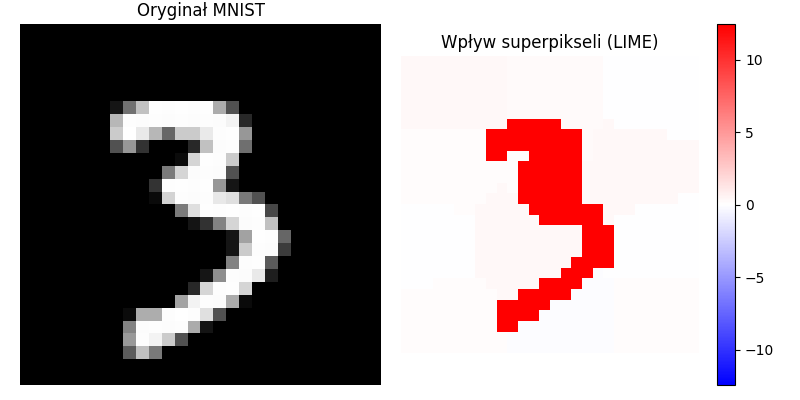
\includegraphics[width=0.45\textwidth]{wyniki_xai/mnist_lime_sample30_class3.png}}
\caption{Atrybucje LIME na cyfrze 3 (próbka 30). Widoczne wzmacniające (czerwone) działanie pętli cyfry.}
\label{fig:mnist_lime_3}
\end{figure}
\begin{figure}[H]
\centerline{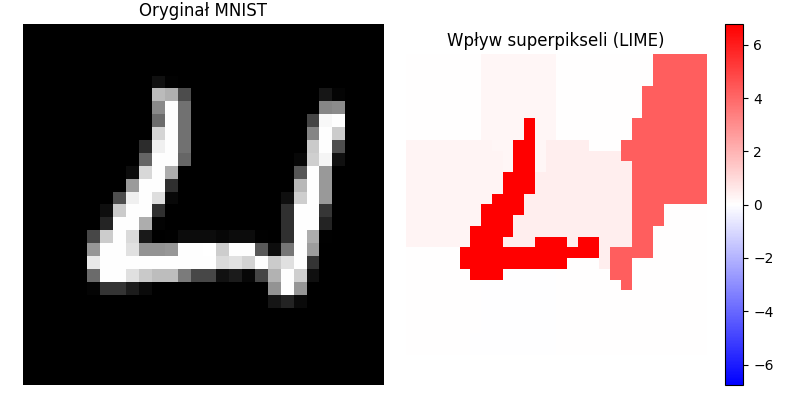
\includegraphics[width=0.45\textwidth]{wyniki_xai/mnist_lime_sample33_class4.png}}
\caption{Atrybucje LIME na cyfrze 4 (próbka 33). Pionowe przecięcia silnie decydują o klasyfikacji na 4.}
\label{fig:mnist_lime_4}
\end{figure}

\begin{figure}[H]
\centerline{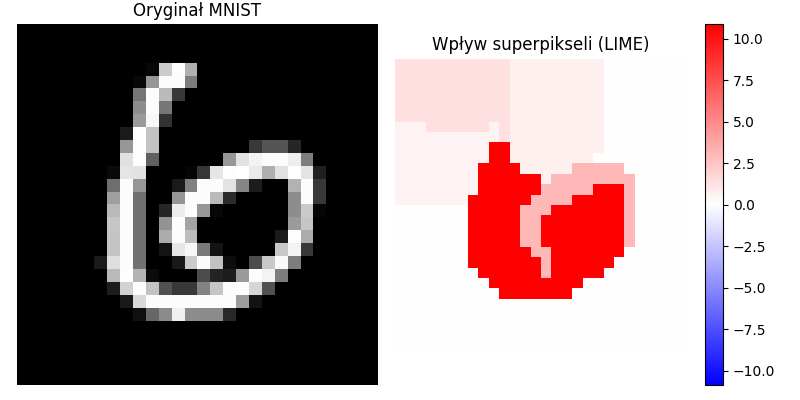
\includegraphics[width=0.45\textwidth]{wyniki_xai/mnist_lime_sample11_class6.png}}
\caption{Atrybucje LIME na cyfrze 6 (próbka 11). Wskazanie na kluczową dla tej klasy pętlę.}
\label{fig:mnist_lime_6}
\end{figure}

\begin{figure}[H]
\centerline{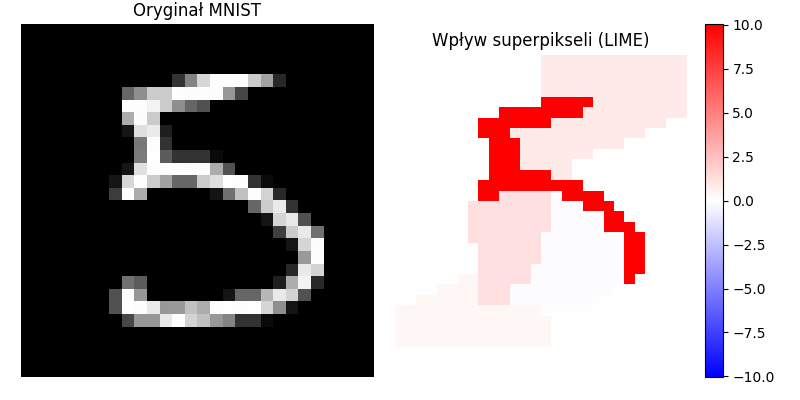
\includegraphics[width=0.45\textwidth]{wyniki_xai/mnist_lime_sample15_class5.png}}
\caption{Atrybucje LIME na cyfrze 5 (próbka 15). Silny wpływ górnego "daszku" oraz dolnego wybrzuszenia.}
\label{fig:mnist_lime_5}
\end{figure}

\subsection{Zbiór obrazowy (Imagenette)}
Dla obrazów naturalnych ze zbioru Imagenette, zastosowanie LIME z segmentacją SLIC (Rys. \ref{fig:imagenette_lime}) pozwoliło na wykazanie, że model skupia swoją uwagę na kluczowych elementach semantycznych obiektów. Wszystkie początkowo analizowane próbki (o indeksach 10, 20, 40 i 90) należą do klasy 0 (,,tench'' - ryba lin).

Na Rys. \ref{fig:imagenette_lime} (próbka 10) czerwone superpiksele o dodatniej atrybucji pokrywają obszar ciała ryby, podczas gdy człowiek trzymający rybę ma ujemną atrybucję (kolor niebieski). W przypadku próbki 20 (Rys. \ref{fig:imagenette_lime_20}) model skupia się na rybie i głowie człowieka trzymającego ją. Dla próbki 40 (Rys. \ref{fig:imagenette_lime_40}) i próbki 90 (Rys. \ref{fig:imagenette_lime_90}) zaobserwowano analogiczne zachowanie: najwyższe dodatnie atrybucje LIME otrzymały segmenty pokrywające ciało ryby, natomiast tło wodne mają znaczenie neutralne lub hamujące. 

Wyniki te dowodzą, że model wykazuje lekkie tendencję do tzw. \textit{shortcut learning} (np. klasyfikowania ryby na podstawie obecności człowieka lub wody w tle), ale również opiera swoje predykcje na poprawnych, biologicznych cechach obiektu.

W celu zbadania zachowania modelu dla innych klas, przeprowadzono analizę LIME dla trzech dodatkowych próbek reprezentujących odmienne kategorie tematyczne ze zbioru Imagenette:
\begin{itemize}
    \item \textbf{Klasa 1 (English springer)} – próbka 387 (Rys. \ref{fig:imagenette_lime_387}): model skupia swoją uwagę (kolor czerwony) bezpośrednio na pyszczku oraz przedniej części ciała psa, podczas gdy trawiaste podłoże ma neutralne i ujemne znaczenie (kolor kremowy i niebieski).
    \item \textbf{Klasa 4 (church)} – próbka 1525 (Rys. \ref{fig:imagenette_lime_1525}): kluczowymi komponentami wspierającymi klasyfikację na kościół są obrysy okien i fasady budynku, lecz nie zwraca on uwagi na wierzę, gdyż jest ona bardzo podobna do tła. Tło nieba oraz otaczające drzewa wykazują neutralną lub ujemną atrybucję, z wyjątkiem jednej gałęzi, która przypomniała modelowi budynek.
    \item \textbf{Klasa 8 (golf ball)} – próbka 3136 (Rys. \ref{fig:imagenette_lime_3136}): dodatnia atrybucja koncentruje się niemal w całości na obszarze w którym znajduje się piłeczka golfowa. Otaczające podłoże trawa wpływa na predykcję modelu, lekko wpływa na wynik modelu, natomiast ujemne znaczenie posiada dół i flaga na polu golfowym.
\end{itemize}
Powyższe obserwacje potwierdzają, że model konwolucyjny z powodzeniem uogólnia istotne cechy wizualne również dla innych kategorii, mimo pewnych wyjątków wynikających ze struktury danych treningowych i próbek, opierając predykcję na kluczowych elementach semantycznych obiektów klasowych.

\begin{figure}[H]
\centerline{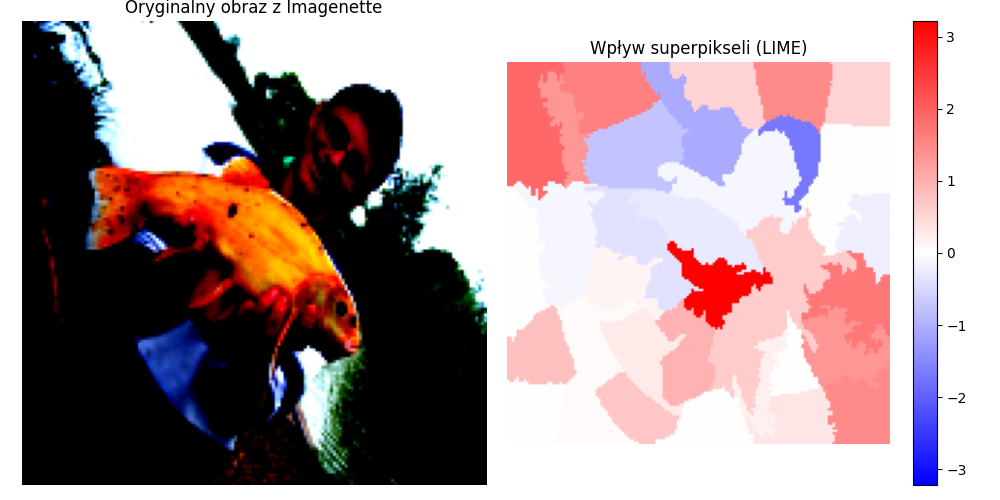
\includegraphics[width=0.45\textwidth]{wyniki_xai/imagenette_lime_sample10_class0.png}}
\caption{Interpretowalne komponenty LIME dla obrazu Imagenette (próbka 10).}
\label{fig:imagenette_lime}
\end{figure}

\begin{figure}[H]
\centerline{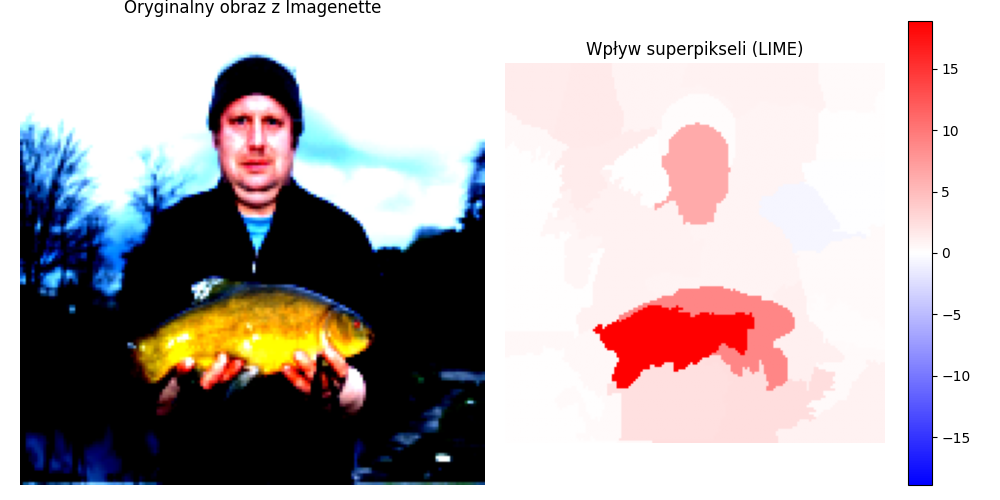
\includegraphics[width=0.45\textwidth]{wyniki_xai/imagenette_lime_sample20_class0.png}}
\caption{Interpretowalne komponenty LIME dla obrazu Imagenette (próbka 20).}
\label{fig:imagenette_lime_20}
\end{figure}

\begin{figure}[H]
\centerline{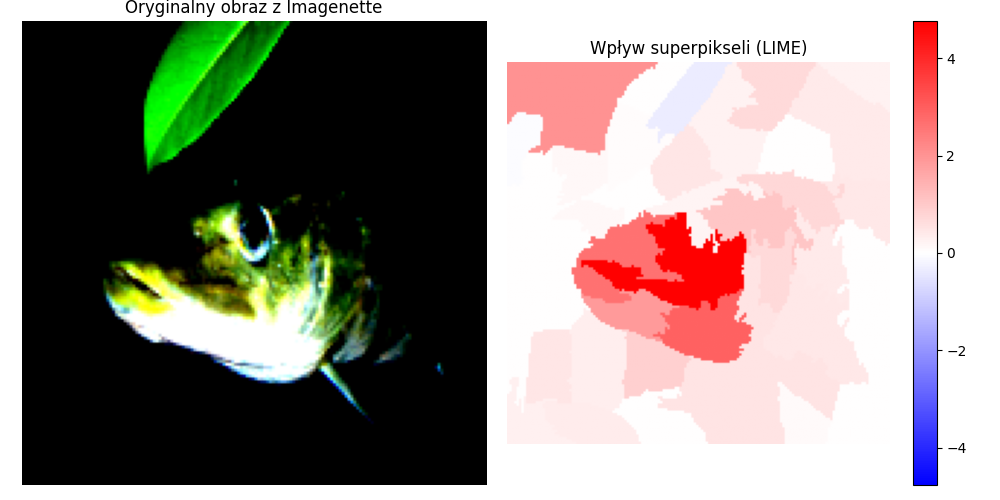
\includegraphics[width=0.45\textwidth]{wyniki_xai/imagenette_lime_sample40_class0.png}}
\caption{Interpretowalne komponenty LIME dla obrazu Imagenette (próbka 40).}
\label{fig:imagenette_lime_40}
\end{figure}

\begin{figure}[H]
\centerline{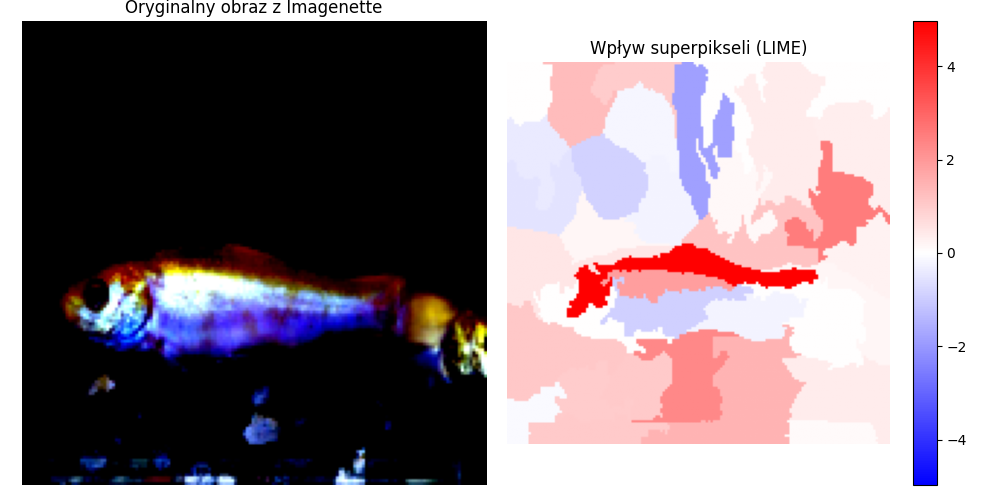
\includegraphics[width=0.45\textwidth]{wyniki_xai/imagenette_lime_sample90_class0.png}}
\caption{Interpretowalne komponenty LIME dla obrazu Imagenette (próbka 90).}
\label{fig:imagenette_lime_90}
\end{figure}

\begin{figure}[H]
\centerline{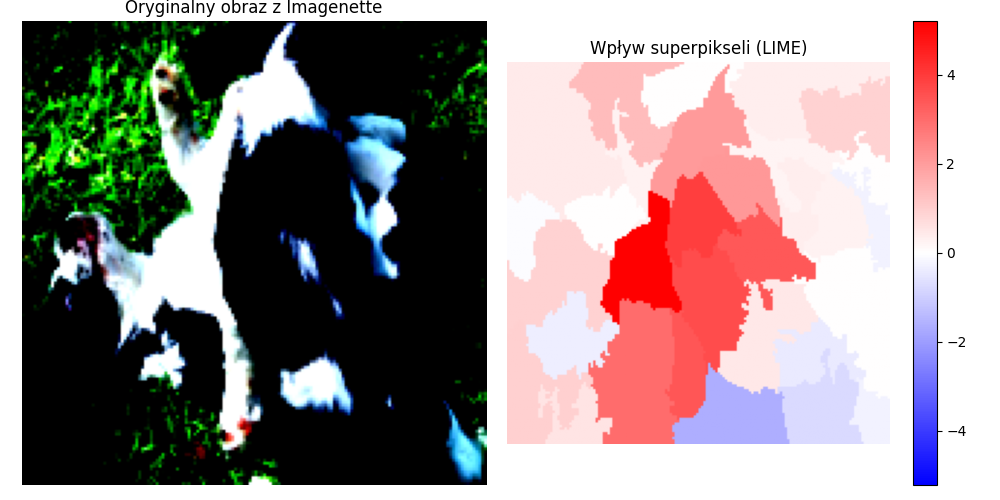
\includegraphics[width=0.45\textwidth]{wyniki_xai/imagenette_lime_sample387_class1.png}}
\caption{Interpretowalne komponenty LIME dla klasy 1 (English springer, próbka 387).}
\label{fig:imagenette_lime_387}
\end{figure}

\begin{figure}[H]
\centerline{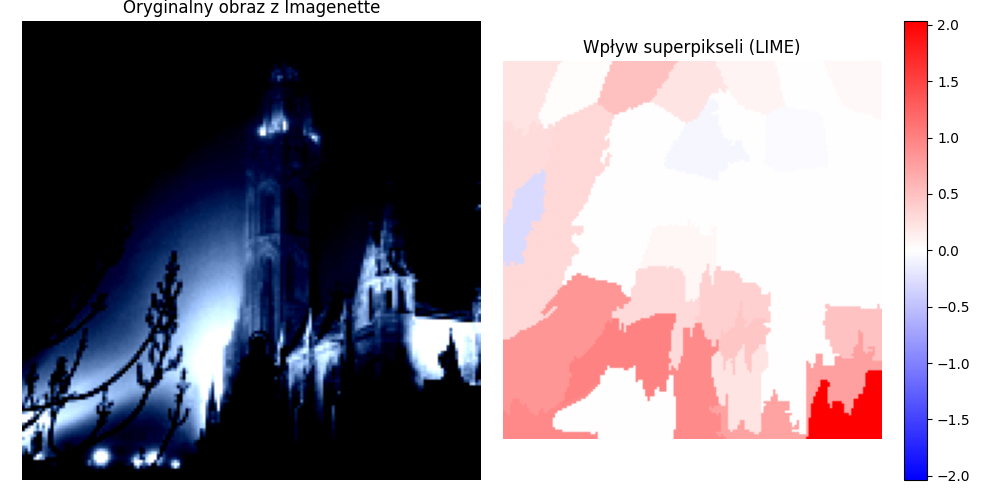
\includegraphics[width=0.45\textwidth]{wyniki_xai/imagenette_lime_sample1525_class4.png}}
\caption{Interpretowalne komponenty LIME dla klasy 4 (church, próbka 1525).}
\label{fig:imagenette_lime_1525}
\end{figure}

\begin{figure}[H]
\centerline{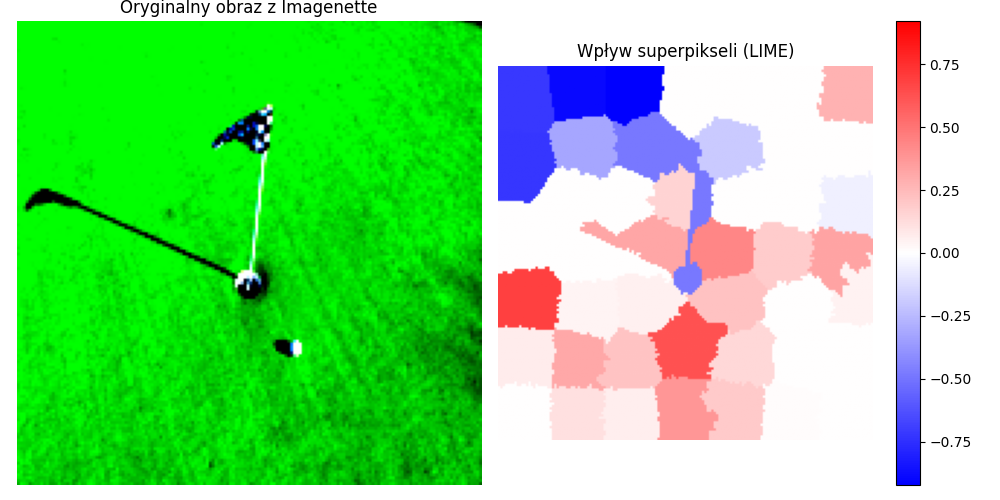
\includegraphics[width=0.45\textwidth]{wyniki_xai/imagenette_lime_sample3136_class8.png}}
\caption{Interpretowalne komponenty LIME dla klasy 8 (golf ball, próbka 3136).}
\label{fig:imagenette_lime_3136}
\end{figure}


\subsection{Globalna interpretacja klas}
Wyniki opisane powyżej dotyczyły pojedynczych próbek. W tej części przedstawiono ujęcie globalne, oparte na wielu przykładach każdej z klas, dla trzech modeli obrazowych.

\subsubsection{MNIST CNN}
Siatka map Saliency (Rys. \ref{fig:mnist_cnn_sal_grid}) potwierdza, że dla pięciu różnych wariantów każdej cyfry model konsekwentnie koncentruje gradienty na rzeczywistym konturze cyfry, a nie na tle. Po uśrednieniu tych map po 60 próbkach na klasę (Rys. \ref{fig:mnist_cnn_sal_mean}) powstaje czytelna globalna sygnatura każdej cyfry: dla klasy 1 dominuje pionowa kreska, dla klasy 0 — pierścień z pustym środkiem, dla klasy 7 — pozioma górna belka wraz ze skosem. Świadczy to, że wysoka skuteczność modelu (98,99\%) wynika z opierania decyzji na powtarzalnych, geometrycznie poprawnych cechach kształtu. Analogiczna siatka dla metody LIME z superpikselami SLIC (Rys. \ref{fig:mnist_cnn_lime_grid}) pokazuje, że dodatnie (czerwone) superpiksele systematycznie pokrywają ślad cyfry niezależnie od próbki.

\subsubsection{MNIST MLP (zoning 4×4)}
Uśredniona atrybucja Feature Ablation zrzutowana na siatkę stref $4\times4$ (Rys. \ref{fig:mnist_mlp_mean}) ujawnia, że uproszczony model tabelaryczny przypisuje każdej cyfrze charakterystyczny, stały rozkład istotnych stref: dla cyfry 1 kluczowa jest środkowa kolumna, dla cyfry 7 — strefa prawego górnego rogu, a dla cyfry 4 — dolno-środkowy obszar przecięcia kresek. Powtarzalność tych wzorców na poziomie pojedynczych próbek dokumentuje siatka przykładów (Rys. \ref{fig:mnist_mlp_grid}). Wyjaśnia to jednocześnie niższą dokładność modelu (85,04\%): reprezentacja 16 stref jest na tyle zgrubna, że sygnatury niektórych par cyfr są do siebie zbliżone.

\subsubsection{Imagenette CNN}
Dla każdej z 10 klas Imagenette wygenerowano siatkę objaśnień LIME (po 5 poprawnie sklasyfikowanych próbek). Przykładowo dla klasy 8 (\textit{golf ball}, Rys. \ref{fig:imagenette_grid_golf}) dodatnia atrybucja powtarzalnie koncentruje się na samej piłeczce, a dla klasy 4 (\textit{church}, Rys. \ref{fig:imagenette_grid_church}) na bryle i fasadzie budynku, przy neutralnym tle nieba. Uzupełniająco, uśredniona mapa Saliency dla wszystkich klas (Rys. \ref{fig:imagenette_sal_mean}) wskazuje, że uwaga modelu jest zogniskowana w centralnym obszarze kadru, gdzie zwykle znajduje się obiekt docelowy. Globalny przegląd wszystkich klas potwierdza więc wcześniejsze wnioski: model w przeważającej mierze opiera predykcje na właściwych obiektach, choć centralne ześrodkowanie uwagi sygnalizuje pewną podatność na położenie obiektu w kadrze.

\begin{figure}[H]
\centerline{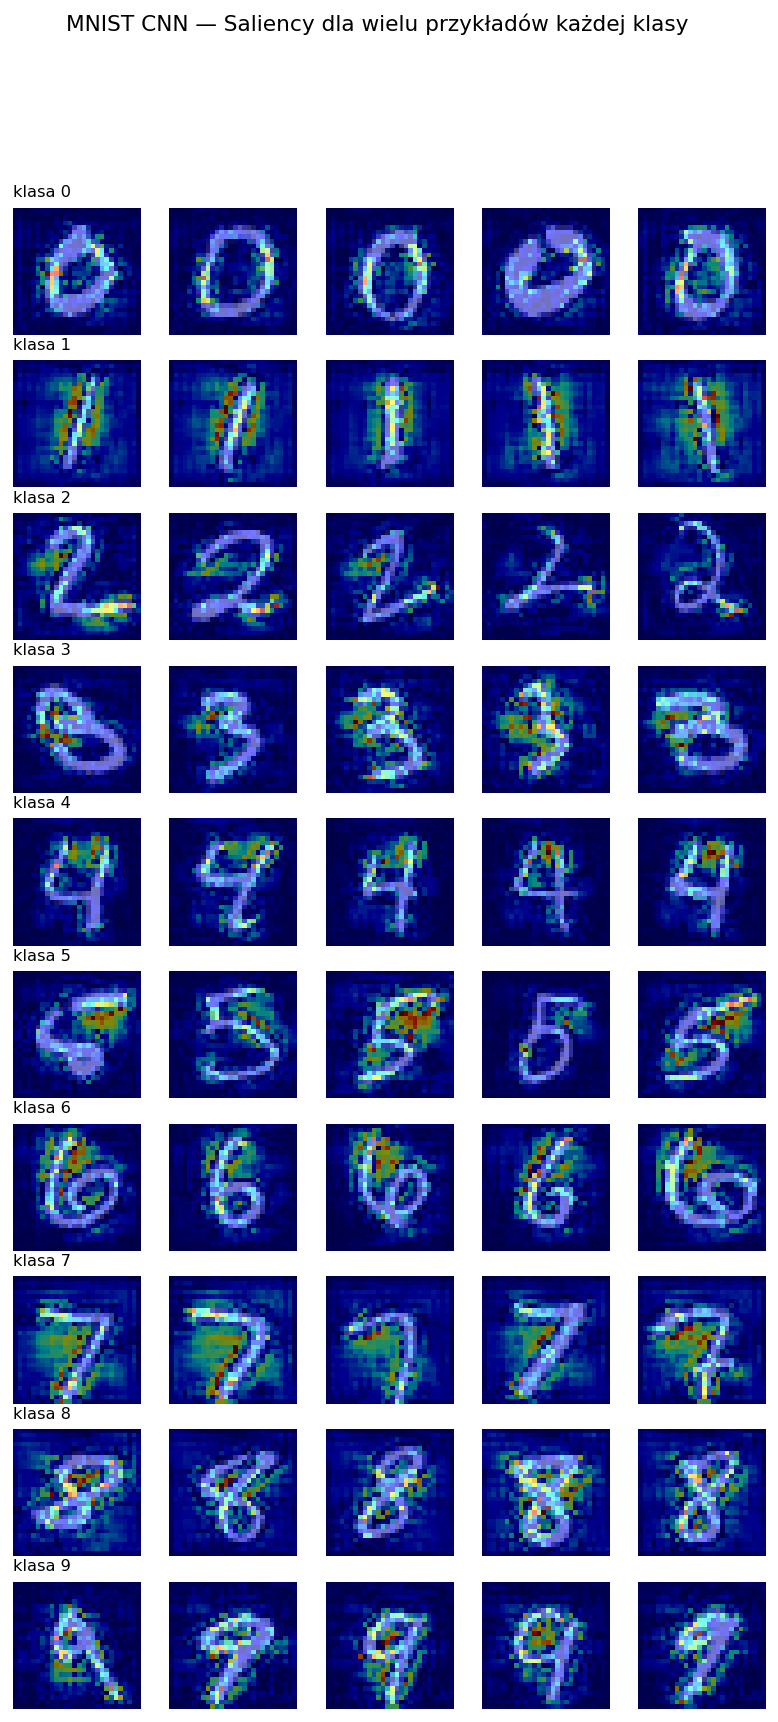
\includegraphics[width=0.42\textwidth]{wyniki_xai/mnist_cnn_saliency_grid_all.png}}
\caption{MNIST CNN — siatka map Saliency dla 5 przykładów każdej z 10 cyfr (wiersze). Uwaga modelu spójnie pokrywa kontur cyfry.}
\label{fig:mnist_cnn_sal_grid}
\end{figure}
\begin{figure}[H]
\centerline{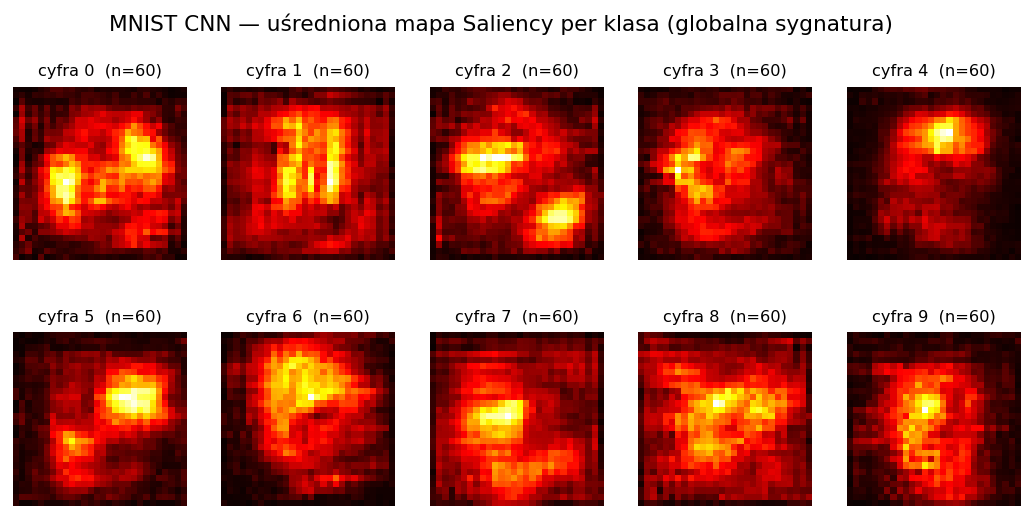
\includegraphics[width=0.48\textwidth]{wyniki_xai/mnist_cnn_saliency_mean_all.png}}
\caption{MNIST CNN — uśredniona mapa Saliency po 60 próbkach na klasę (globalna sygnatura każdej cyfry).}
\label{fig:mnist_cnn_sal_mean}
\end{figure}
\begin{figure}[H]
\centerline{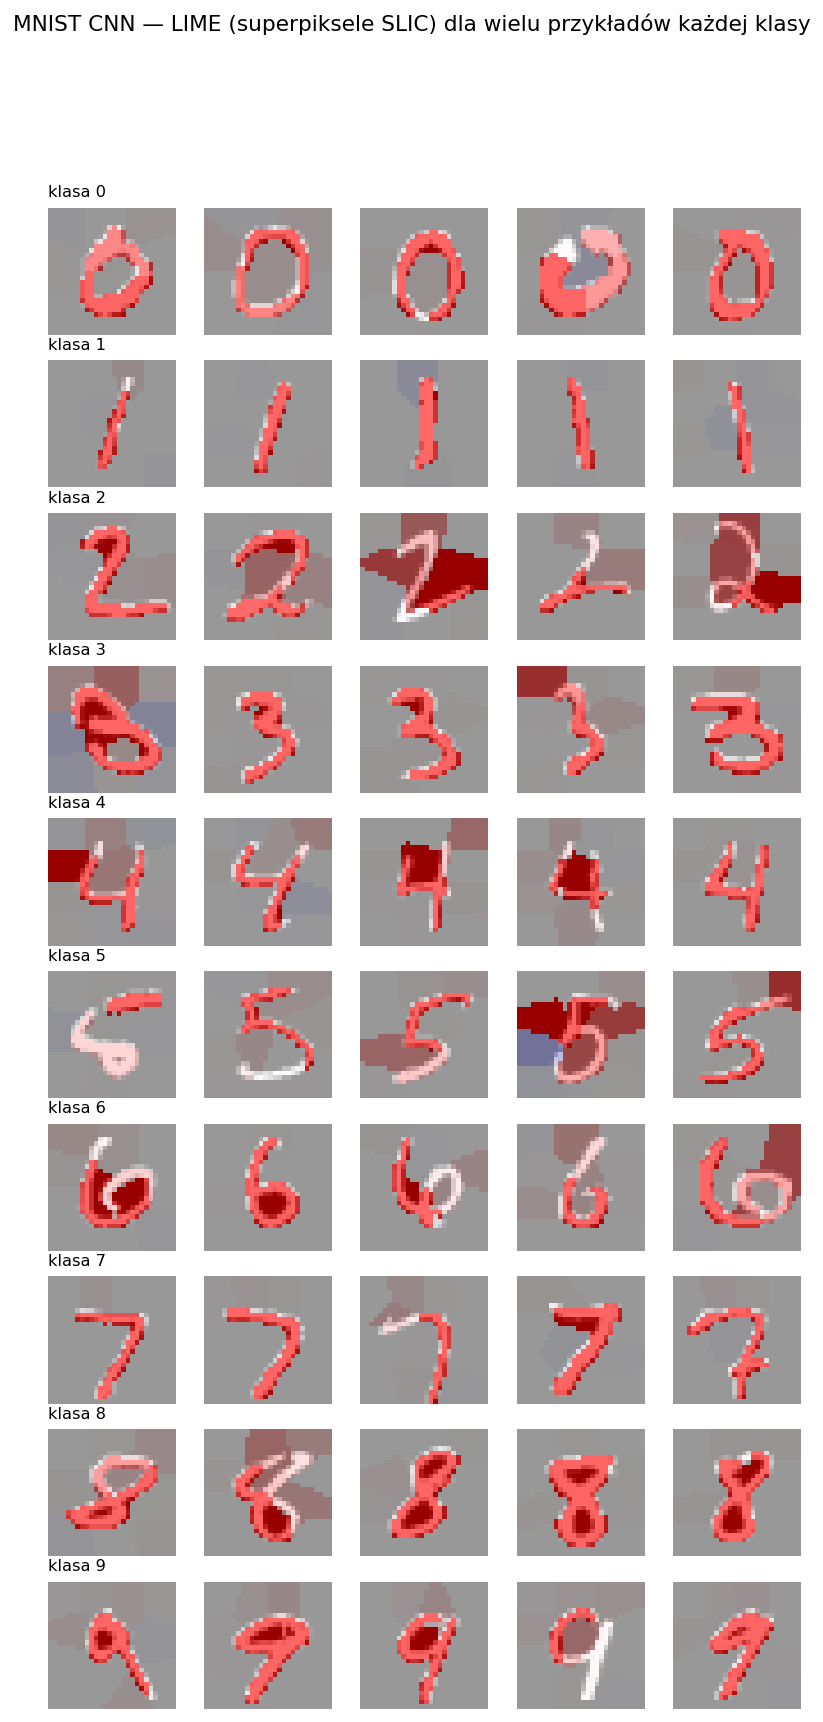
\includegraphics[width=0.42\textwidth]{wyniki_xai/mnist_cnn_lime_grid_all.png}}
\caption{MNIST CNN — siatka objaśnień LIME (SLIC) dla 5 przykładów każdej cyfry.}
\label{fig:mnist_cnn_lime_grid}
\end{figure}
\begin{figure}[H]
\centerline{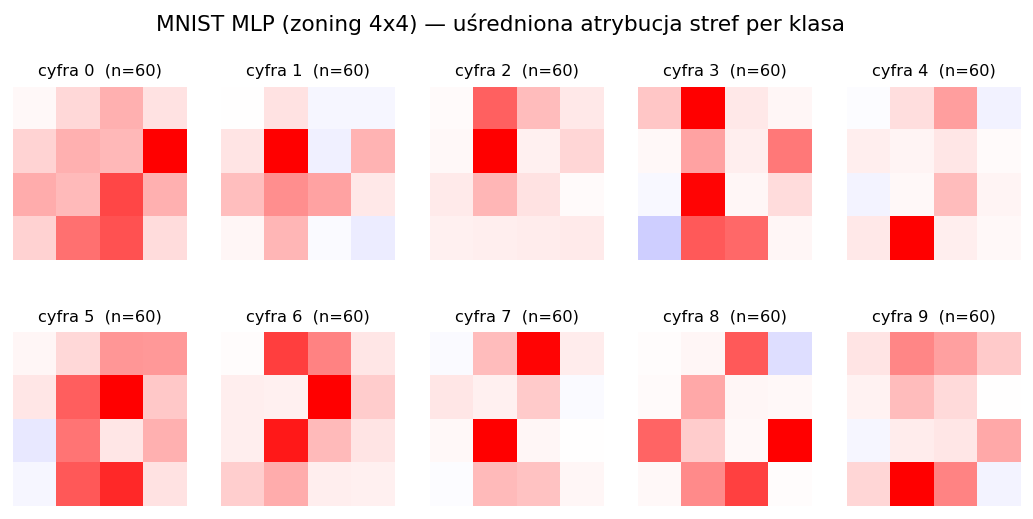
\includegraphics[width=0.48\textwidth]{wyniki_xai/mnist_mlp_zoning_mean_all.png}}
\caption{MNIST MLP (zoning) — uśredniona atrybucja stref $4\times4$ na klasę. Każda cyfra ma odrębny rozkład istotnych stref.}
\label{fig:mnist_mlp_mean}
\end{figure}
\begin{figure}[H]
\centerline{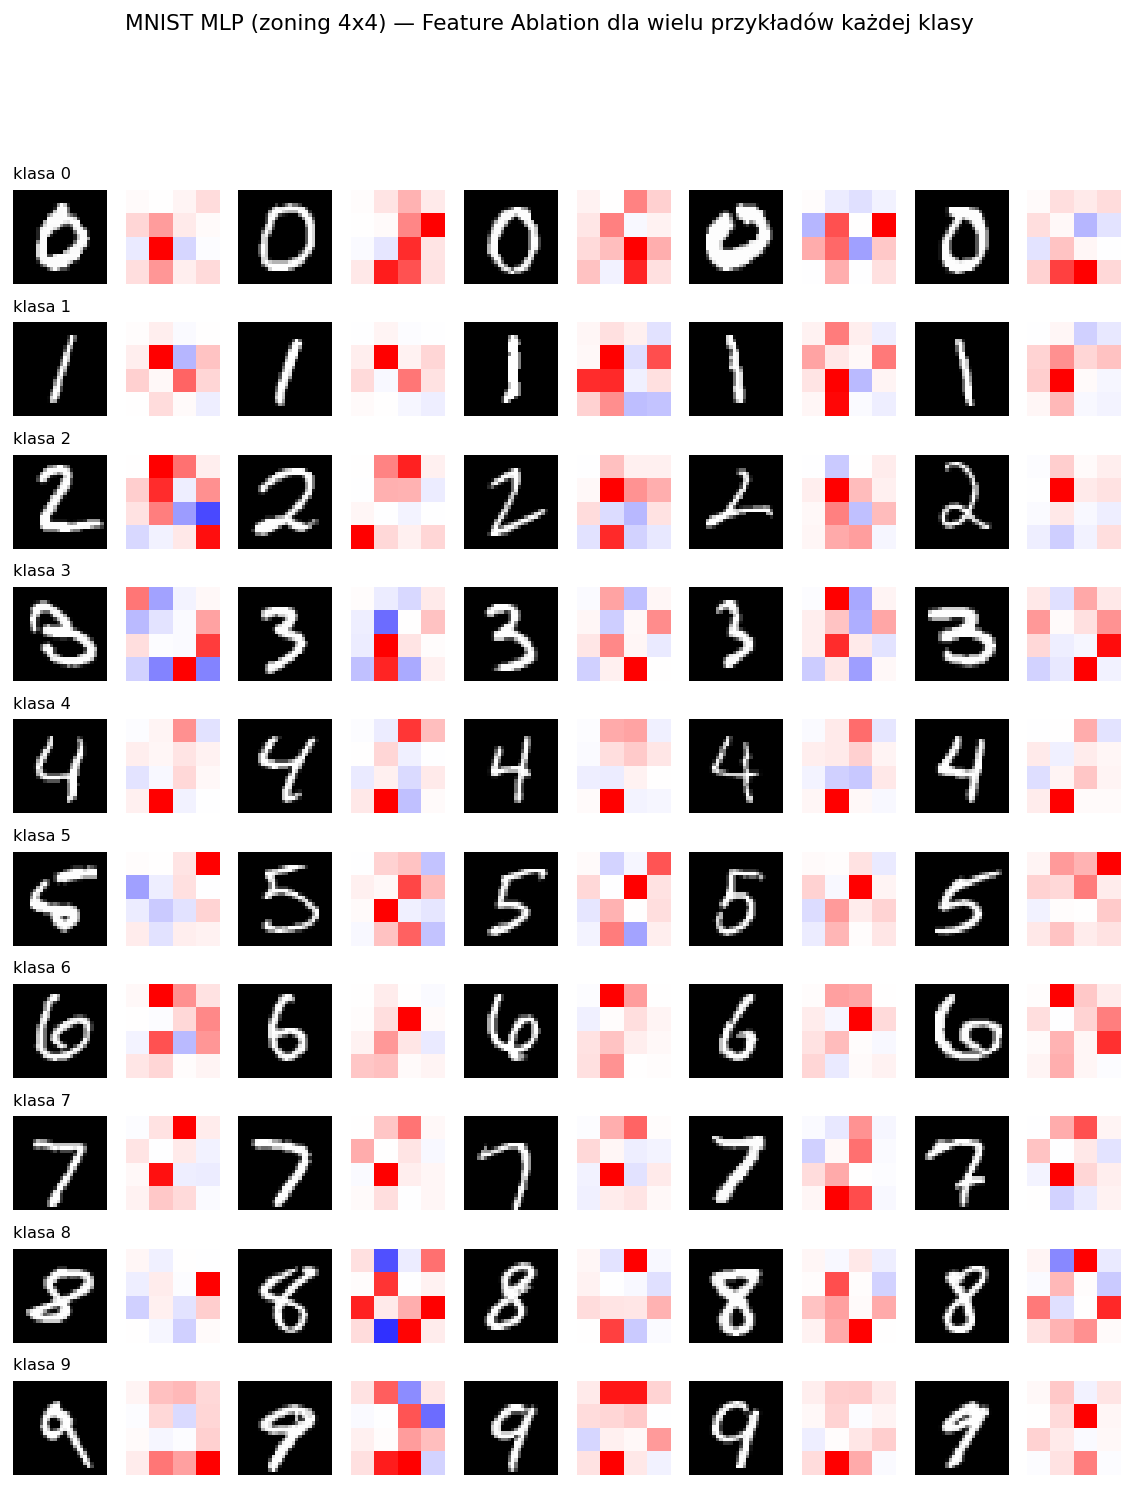
\includegraphics[width=0.48\textwidth]{wyniki_xai/mnist_mlp_zoning_grid_all.png}}
\caption{MNIST MLP (zoning) — siatka: oryginał oraz mapa stref $4\times4$ dla 5 przykładów każdej cyfry.}
\label{fig:mnist_mlp_grid}
\end{figure}
\begin{figure}[H]
\centerline{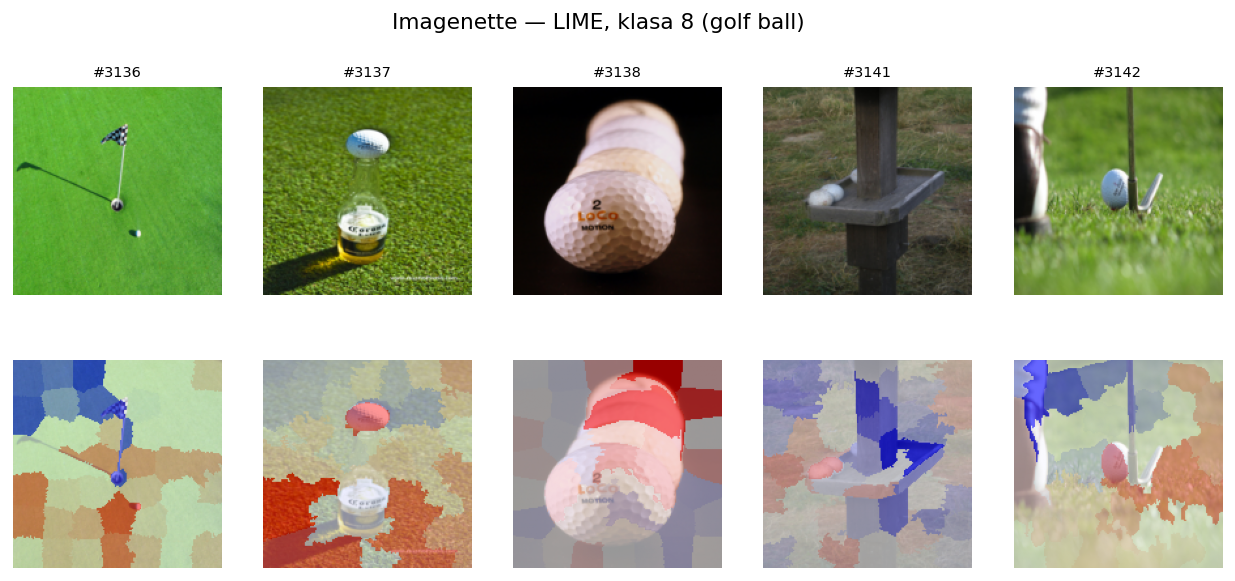
\includegraphics[width=0.48\textwidth]{wyniki_xai/imagenette_lime_grid_class8.png}}
\caption{Imagenette — siatka LIME dla klasy 8 (\textit{golf ball}). Atrybucja powtarzalnie wskazuje piłeczkę.}
\label{fig:imagenette_grid_golf}
\end{figure}
\begin{figure}[H]
\centerline{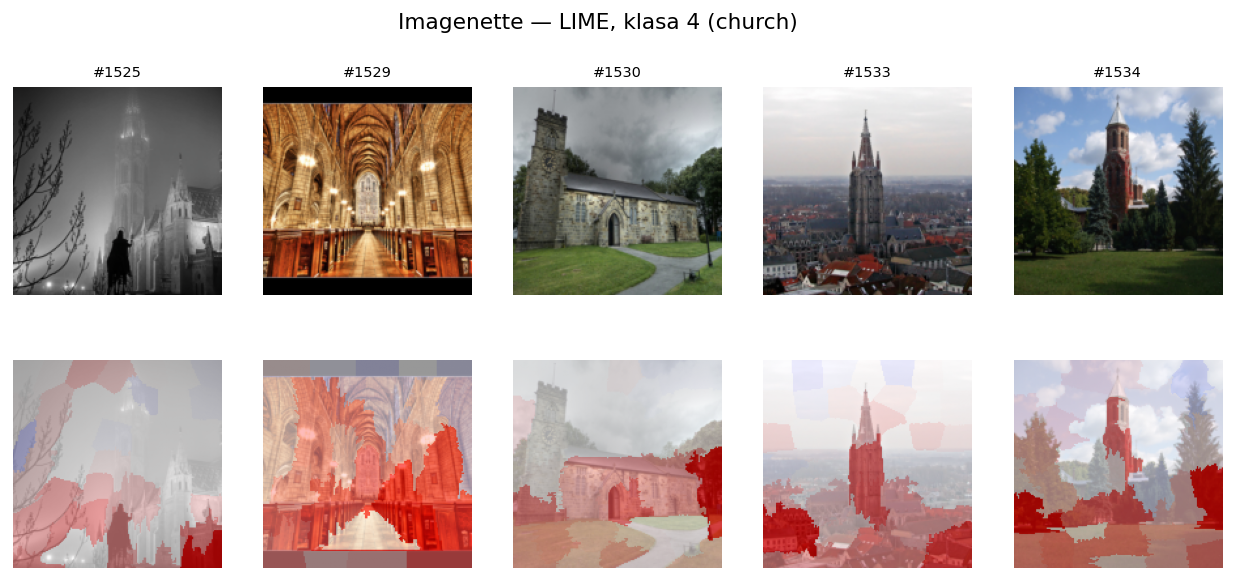
\includegraphics[width=0.48\textwidth]{wyniki_xai/imagenette_lime_grid_class4.png}}
\caption{Imagenette — siatka LIME dla klasy 4 (\textit{church}). Atrybucja koncentruje się na bryle budynku.}
\label{fig:imagenette_grid_church}
\end{figure}
\begin{figure}[H]
\centerline{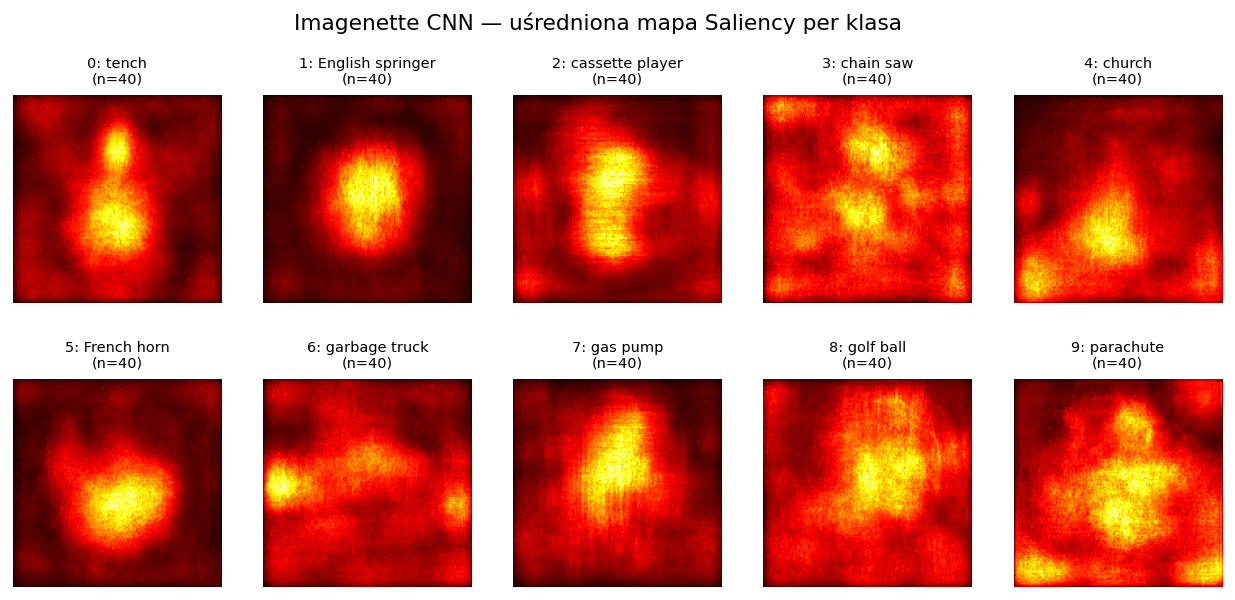
\includegraphics[width=0.48\textwidth]{wyniki_xai/imagenette_saliency_mean_all.png}}
\caption{Imagenette CNN — uśredniona mapa Saliency per klasa (uwaga zogniskowana w centrum kadru).}
\label{fig:imagenette_sal_mean}
\end{figure}


\section{Podsumowanie (Summary)}
Przeprowadzone eksperymenty na modelach sieci neuronowych (MLP oraz CNN) z wykorzystaniem biblioteki Captum potwierdziły wysoką użyteczność metod Objaśnialnej Sztucznej Inteligencji w analizie struktur decyzyjnych modeli typu ,,czarna skrzynka''. Dzięki zastosowaniu zróżnicowanych algorytmów (Feature Ablation, Saliency Maps, LIME, perturbacji kierunkowych) możliwe było spojrzenie na zachowanie sieci z wielu komplementarnych perspektyw.

Główne wnioski wynikające z przeprowadzonych badań obejmują:
\begin{itemize}
    \item \textbf{Zbieżność metod:} Objaśnienia generowane przez metody gradientowe (Saliency) oraz perturbacyjne (LIME, Ablation) wykazują dużą zgodność przestrzenną. Kluczowe cechy geometryczne (np. pętle w MNIST) oraz atrybuty chemiczne (np. prolina dla Wine) są spójnie wskazywane jako najważniejsze elementy decyzyjne.
    \item \textbf{Ocena odporności:} Behawioralna analiza perturbacyjna pozwoliła wyznaczyć fizyczne granice decyzyjne modeli. Wyznaczenie punktów krytycznych (np. $h_{crit}=18$ dla cyfry 4) dostarcza intuicyjnych, zrozumiałych dla człowieka informacji o wrażliwości klasyfikatora na zniekształcenia geometryczne.
    \item \textbf{Identyfikacja shortcut learning:} Metoda LIME z superpikselami SLIC na zbiorze Imagenette potwierdziła skupienie uwagi modelu na obiektach docelowych, co minimalizuje ryzyko błędnego działania systemu w warunkach produkcyjnych.
    \item \textbf{Globalne sygnatury klas:} Agregacja objaśnień po wielu próbkach (siatki oraz mapy uśrednione) wykazała, że modele stosują spójne, powtarzalne wzorce decyzyjne dla każdej klasy. Uśrednione mapy Saliency oraz atrybucji stref tworzą czytelne ,,sygnatury'' klas, przenosząc analizę z poziomu pojedynczej próbki na poziom globalnego zachowania modelu.
\end{itemize}

\subsection{Kierunkowa analiza przyszłych prac}
W ramach dalszego rozwoju podjętej tematyki planuje się realizację następujących zagadnień:
\begin{enumerate}
    \item \textbf{Badanie nowoczesnych architektur:} Zastosowanie metod XAI do analizy modeli opartych na mechanizmie uwagi, takich jak Vision Transformers (ViT) czy sieci grafowe (GNN).
    \item \textbf{Ilościowa ocena objaśnień:} Wprowadzenie metryk oceny wiarygodności atrybucji, np. poprzez wyznaczanie krzywych usuwania i wstawiania cech oraz badanie wierności lokalnej.
    \item \textbf{Trening sterowany objaśnieniami:} Wykorzystanie map atrybucji do nakładania kar regularyzacyjnych na gradienty w procesie uczenia (ang. \textit{explanation-guided learning}) w celu eliminacji podatności modelu na nieistotne korelacje tła.
    \item \textbf{Interaktywne interfejsy XAI:} Opracowanie pulpitów nawigacyjnych (dashboards) umożliwiających użytkownikom końcowym dynamiczne modyfikowanie cech i natychmiastowy podgląd zmian atrybucji lokalnych.
\end{enumerate}


\appendices
\section{Parametry i trening modeli klasyfikacyjnych}
Wszystkie modele zostały zaimplementowane w bibliotece PyTorch i wytrenowane na procesorach graficznych (CUDA). Specyfikacja parametrów treningowych przedstawia się następująco:
\begin{itemize}
    \item \textbf{Modele MLP (Iris, Wine):} Architektura z jedną warstwą ukrytą (16 i 26 neuronów, aktywacja ReLU). Optymalizator: Adam ze współczynnikiem uczenia $\eta = 0.01$. Trening prowadzony przez 100 epok przy minimalizacji straty Cross-Entropy.
    \item \textbf{Model MLP MNIST (zoning16):} Wejście zredukowane do 16 cech (strefowanie). Warstwa ukryta: 32 neurony. Trening: optymalizator Adam ($\eta = 0.005$), 50 epok.
    \item \textbf{Model CNN MNIST:} Dwie warstwy konwolucyjne ($3 \times 3$, filtry 32 i 64) z warstwami MaxPool $2 \times 2$ i warstwą w pełni połączoną (128 neuronów). Optymalizator: Adam ($\eta = 0.001$), 10 epok, rozmiar paczki (batch size): 64.
    \item \textbf{Model CNN Imagenette:} Architektura bazująca na standardowym modelu ResNet-18. Optymalizator: SGD z pędem (momentum = 0.9) oraz współczynnikiem uczenia $\eta = 0.001$ z tłumieniem wag (weight decay = $10^{-4}$). Prowadzony przez 15 epok z paczkami o rozmiarze 32.
\end{itemize}

\section{Konfiguracja metod XAI i segmentacji}
Do generowania objaśnień wykorzystano następujące nastawy algorytmów:
\begin{itemize}
    \item \textbf{Feature Ablation:} Użyto zerowej próbki bazowej (wektor zerowy $\mathbf{0}$).
    \item \textbf{SLIC (Simple Linear Iterative Clustering):}
    \begin{itemize}
        \item \textit{MNIST:} Liczba superpikseli $d = 15$, współczynnik zwartości (compactness) $= 10.0$. Obrazy jednokanałowe przed segmentacją poddano lekkiemu wygładzeniu filtrem Gaussa ($\sigma = 0.5$).
        \item \textit{Imagenette:} Liczba superpikseli $d = 50$, współczynnik zwartości $= 10.0$.
    \end{itemize}
    \item \textbf{LIME:} Liczba perturbacji losowych $N = 1000$ próbek dla każdego objaśnienia. Do wyznaczania wag bliskości użyto jądra wykładniczego o szerokości pasma (kernel width) równej $0.75$. W charakterze lokalnego modelu interpretowalnego wyuczono regresję Lasso z celem wyselekcjonowania maksymalnie 10 kluczowych cech (superpikseli).
\end{itemize}

% references section
\begin{thebibliography}{00}
\bibitem{Ribeiro2016} M. T. Ribeiro, S. Singh, and C. Guestrin, ``Why Should I Trust You?'': Explaining the Predictions of Any Classifier, in \textit{Proceedings of the 22nd ACM SIGKDD International Conference on Knowledge Discovery and Data Mining}, San Francisco, CA, USA, pp. 1135--1144, 2016.
\bibitem{Simonyan2013} K. Simonyan, A. Vedaldi, and A. Zisserman, ``Deep Inside Convolutional Networks: Visualising Image Classification Models and Saliency Maps,'' \textit{arXiv preprint arXiv:1312.6034}, 2013.
\bibitem{Wachter2017} S. Wachter, B. Mittelstadt, and C. Russell, ``Counterfactual explanations without opening the black box: Automated decisions and the GDPR,'' \textit{Harvard Journal of Law \& Technology}, vol. 31, no. 2, pp. 841--887, 2018.
\bibitem{Zeiler2014} M. D. Zeiler and R. Fergus, ``Visualizing and understanding convolutional networks,'' in \textit{European Conference on Computer Vision (ECCV)}, Zurich, Switzerland, pp. 818--833, 2014.
\end{thebibliography}

% that's all folks
\end{document}
